
\documentclass{article}
\usepackage[spanish]{babel} %Definir idioma español
\usepackage[utf8]{inputenc} %Codificacion utf-8
\usepackage{amssymb, amsmath, amsbsy, wasysym}
\usepackage{multirow} % para tablas
\usepackage{graphicx}
\author{Emmanuel Peto Gutiérrez}
\title{Práctica 1: Merge sort\\Computación distribuida}
\begin{document}
\maketitle

\section{Ejecución}

Para compilar y correr el programa se debe ejecutar el comando \texttt{make} desde la terminal, lo cual corre el programa con 8 hilos. Cuando ya está compilado, si se quiere ejecutar otra vez se hace con:

\texttt{mpirun -n <número de hilos> MSparalelo} Para ejecutarlo con un número determinado de hilos.

\texttt{mpirun MSparalelo} Para ejecutarlo con el número de procesadores disponibles en la red o computadora.

\section{Comunicación}

La comunicación entre nodos se realiza en forma de árbol binario: un nodo le envía mensajes a sus hijos o a su padre. Como el número de nodos puede variar se arreglan en forma de Heap, donde la raíz es el procesador con rango 0. Si un nodo tiene rango $i$, su hijo izquierdo es el $2i+1$, el derecho el $2i+2$ y el padre el $\lfloor (i-1)/2 \rfloor$.

En MPI se puede enviar un mensaje a cualquier nodo, pero en el algoritmo solo se utilizan las aristas mostradas en la figura \ref{heap} en un ejemplo de 10 procesos.

\begin{figure}[htbp]
\begin{center}
\includegraphics[scale=1]{red1}
\caption{Comunicación de árbol.}
\label{heap}
\end{center}
\end{figure}

La forma en la que se comunican y las operaciones que realizan depende de la ubicación del nodo en el árbol, y para esto se definen cuatro tipos de nodos:

\begin{itemize}
\item Raíz: es la raíz del árbol y siempre será el proceso con rango 0.
\item Interno: es un nodo no raíz que tiene hijo izquierdo e hijo derecho.
\item Semi-interno: tiene un hijo izquierdo pero no derecho. De este tipo puede existir a lo más uno.
\item Hoja: no tiene hijo izquierdo ni derecho. Se encuentran al fondo del árbol.
\end{itemize}

\section{Algoritmo}

Como se sabe, \textit{merge sort} consta de dos partes: partir (split) y fusionar (merge). 

\subsection*{Split}

El nodo raíz inicia el proceso partiendo la entrada en dos y envía cada parte a sus hijos. Un nodo interno espera el mensaje de su padre (que es un arreglo), parte este arreglo en dos y lo envía a sus hijos; si se llegó al caso base en el que el arreglo tiene tamaño 1 ya no se parte pero se tiene que enviar algo a sus hijos, pues todos los nodos que no son la raíz están esperando un mensaje. El nodo semi-interno envía la parte izquierda del arreglo a su hijo izquierdo y ordena la parte derecha usando merge sort secuencial. Finalmente, un nodo hoja ordena el arreglo que recibió usando merge sort secuencial.

La comunicación se realiza de la raíz hacia las hojas como se muestra en la figura \ref{split}.

\begin{figure}[htbp]
\begin{center}
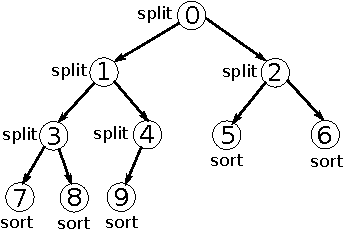
\includegraphics[scale=1]{red2}
\caption{Proceso de partir.}
\label{split}
\end{center}
\end{figure}

\subsection*{Merge}

Cuando ya se tiene un arreglo ordenado en una hoja, este se manda de vuelta a su padre. Los nodos internos esperan dos mensajes, que son dos arreglos ordenados; al recibirlos los fusionan con el algoritmo merge secuencial y envían el resultado a su padre. La diferencia con el semi-interno es que este solo espera un mensaje, pero también utiliza el algoritmo merge. Finalmente, la raíz recibe dos arreglos ordenados y los fusiona.

La comunicación se realiza de las hojas hacia la raíz como se muestra en la figura \ref{merge}.

\begin{figure}[htbp]
\begin{center}
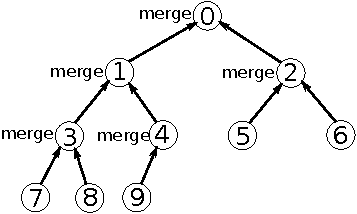
\includegraphics[scale=1]{red3}
\caption{Proceso de fusionar.}
\label{merge}
\end{center}
\end{figure}

\end{document}

